\documentclass[lualatex,hyperref={pdfencoding=auto}]{beamer}
\usepackage[czech]{babel}
% \usepackage[utf8]{inputenc}
\usepackage{biblatex}
\usepackage{algorithm}
\usepackage{algorithmic}
% \usepackage{graphicx}
\addbibresource{citace.bib}
\usetheme[fei]{vsb}



\usepackage{tikz}
\usetikzlibrary{positioning,calc}

% \bibliography{citace.bib}

% \addbibresource{citace.bib}

\title[Komprese stromových struktur]{Komprese stromových struktur}
\subtitle{Semestrální projekt}
\author{Marek Beran}
\institute[VŠB-TUO]{VŠB -- Technická univerzita Ostrava\\\vspace{2mm}marek.beran.st@vsb.cz}
\date[27.~5.~2025]{27.~května 2025}

\showboxdepth=5

\begin{document}

\section{Úvod}

\begin{frame}{Obsah}
    \tableofcontents
\end{frame}

\begin{frame}{Cíl a motivace}

\begin{itemize}
    \item Je možné efektivně komprimovat přirozený jazyk převedením do stromové struktury?
    \item Cíl: Proof of Concept
\end{itemize}
\end{frame}

% \section{Implementace knihovny}
% \begin{frame}{Použité technologie}
%     \begin{columns}[t] 
%         \begin{column}{0.5\textwidth}
%             \vspace{0pt} % Vynucení zarovnání nahoře
%             \textbf{Programovací jazyk a platforma:}
%             \begin{itemize}
%                 \item C\# 9.0
%                 \item .NET 5.0 a vyšší
%                 \item Visual Studio 2022
%             \end{itemize}
%             \vspace{12pt}
%             \textbf{Knihovny:}
%             \begin{itemize}
%                 \item UDPipe 
%                 (rozpoznávání syntaktických stromů) \nocite{udpipe:2017}
%                 \item MorphoDiTa (morfologická analýza) \nocite{strakova14}
%             \end{itemize}
%         \end{column}
%         \begin{column}{0.5\textwidth}
%             \vspace{0pt} % Vynucení zarovnání nahoře
%             \textbf{Další nástroje:}
%             \begin{itemize}
%                 \item R (datová analýza a vizualizace)
%                 \item Mkdocs (dokumentace)
%                 \item Bash skripty (podpůrné nástroje)
%             \end{itemize}
            
%             \textbf{Bindings:}
%             \begin{itemize}
%                 \item C\# wrapper pro UDPipe (nativní knihovna) 
%                 \item C\# wrapper pro MorphoDiTa (nativní knihovna) 
%             \end{itemize}
%         \end{column}
%     \end{columns}
% \end{frame}


\begin{frame}{Implementace knihovny}
  \nocite{Oquendo2016Pipe}
    \begin{figure}
        \centering
        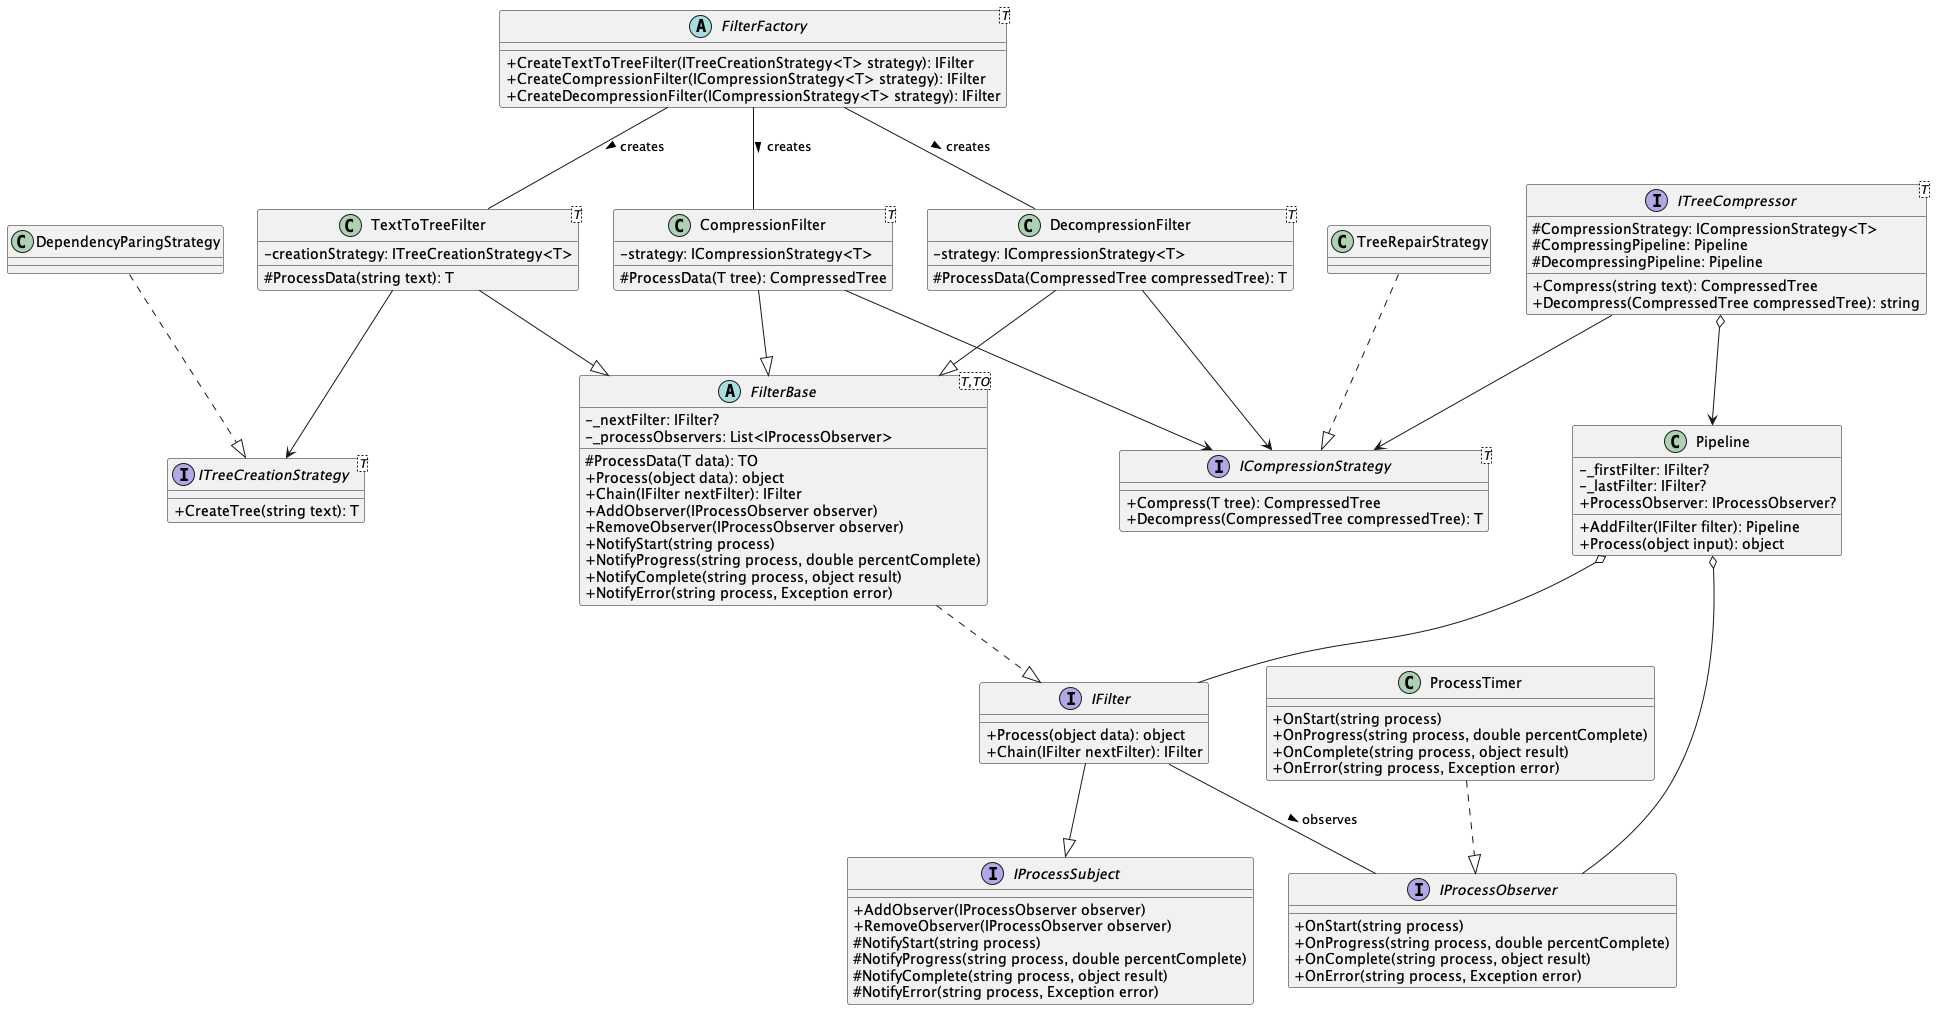
\includegraphics[width=\textwidth]{fig/class-diagram.png}
        \caption{Třídní diagram části implementace zaměření na řetězení filtrů}
        \label{fig:class-diagram}
    \end{figure}
\end{frame}

\section{Převod textu do stromové struktury}

\begin{frame}{Převod textu do stromové struktury}
  \begin{itemize}
    \item Dependency parsing - závislosti mezi slovy ve větě.\nocite{kubler2009dependency} \nocite{jurafsky2024speech} \nocite{filippova2008dependency}
    \item Využití knihovny UDPipe pro syntaktickou analýzu textu
    \item Vytvoření syntaktického stromu pro každou větu
  \end{itemize}
  \centering
  \begin{tikzpicture}[
% Node styles
 box/.style={draw, rounded corners, fill=blue!10, font=\sffamily,
 minimum width=1.2cm, minimum height=0.8cm, align=center},
 root/.style={fill=blue!20},
% Edge styles
 edge/.style={draw, thick, black!50},
% Label styles
 label/.style={midway, font=\small\sffamily}
]
% Root node
\node[box, root] (jumps) at (0,0) {jumps};
% Left branch (fox and children)
\node[box] (fox) at (-2,-1) {fox};
\node[box] (the) at (-6.6,-3) {The};
\node[box] (quick) at (-4.6,-3) {quick};
\node[box] (brown) at (-2.6,-3) {brown};
% Right branch (over and descendants)
\node[box] (dog) at (3,-3) {dog};
\node[box] (over) at (-2,-5) {over};
\node[box] (the2) at (0,-5) {the};
\node[box] (lazy) at (2,-5) {lazy};
% Connect nodes with edges
\draw[edge] (jumps) -- (fox) node[label, left] {nsubj};
\draw[edge] (fox) -- (the) node[label, left] {det};
\draw[edge] (fox) -- (quick) node[label, left] {amod};
\draw[edge] (fox) -- (brown) node[label, right] {amod};
\draw[edge] (jumps) -- (dog) node[label, right] {case};
\draw[edge] (dog) -- (over) node[label, left] {obl};
\draw[edge] (dog) -- (the2) node[label, left] {det};
\draw[edge] (dog) -- (lazy) node[label, right] {amod};
\end{tikzpicture}
\end{frame}

\begin{frame}{Umělé rozšíření stromu}
  \begin{itemize}
    \item Rozšíření stromu pro podporu více vět bez nutnosti práce s lesem
    \item Pro zajištění dostatečné velikosti syntaktického stromu pro testování a kompresi
  \end{itemize}
  \centering
    \begin{tikzpicture}[
% Node styles
 box/.style={draw, rounded corners, fill=blue!10, font=\sffamily,
 minimum width=1.2cm, minimum height=0.8cm, align=center},
 root/.style={fill=blue!20},
% Edge styles
 edge/.style={draw, thick, black!50},
% Label styles
 label/.style={midway, font=\small\sffamily}
]
\node[box] (document) at (0,0) {<Document>};

\node [box] (root1) at (-3,-3) {<Root>};
\node [box] (root2) at (-1,-3) {<Root>};
\node [box] (root3) at (1,-3) {<Root>};
\node [box] (root4) at (3,-3) {<Root>};

\draw[edge] (document) -- (root1);
\draw[edge] (document) -- (root2);
\draw[edge] (document) -- (root3);
\draw[edge] (document) -- (root4);

\draw[edge, opacity=0.3] (document) -- ++(-5, -2.5);
\draw[edge, opacity=0.3] (document) -- ++(5, -2.5);

\draw[edge, opacity=0.3] (root1) -- ++(0, -1);
\draw[edge, opacity=0.3] (root2) -- ++(0, -1);
\draw[edge, opacity=0.3] (root3) -- ++(0, -1);
\draw[edge, opacity=0.3] (root4) -- ++(0, -1);

\node at (-5,-3) {\Huge$\cdots$};
\node at (5,-3) {\Huge$\cdots$};


\node at (-3,-4.2) {\Huge$\vdots$};
\node at (-1,-4.2) {\Huge$\vdots$};
\node at (1,-4.2) {\Huge$\vdots$};
\node at (3,-4.2) {\Huge$\vdots$};

\end{tikzpicture}
\end{frame}

\section{Algoritmy}
\begin{frame}{Algoritmy}
  \begin{itemize}
    \item Zaměření na gramatickou kompresi
    \item Zpočátku exaktní metody (generování hashů pro všechny podstromy)
    \item Komprimace pomocí linearizace -- převod stromu na posloupnost uzlů a jejich následná komprese pomocí algoritmů pro kompresi textu \nocite{McAnlis2016}
    \item Pokus o optimalizaci linearizovaného RePair (Recursive Pairing) algoritmu pro kompresi linearizovaných stromových struktur (maximální komprimace redundantních struktur) -- hledání n-tic
    \item Komprese bez linearizace -- algoritmus pro kompresi stromových struktur inspirovaný RePair algoritmem 
    \item Opět pokus o optimalizaci
  \end{itemize}
\end{frame}

\begin{frame}{Pseudokód algoritmu}
\begin{algorithm}[H]
\caption{Algoritmus pro kompresi bez linearizace} 
\begin{algorithmic}[1] 
  \REQUIRE Závislostní strom $T$ 
  \STATE Inicializuj čítač pravidel a slovník digramů 
  \STATE Projdi strom a vytvoř index všech digramů $(\text{rodič}, \text{dítě}, \text{pozice})$ 
  \WHILE{existuje digram $D$ s četností $\geq 2$} 
  \STATE Najdi digram $D$ s nejvyšší četností 
  \STATE Vytvoř nový neterminál $N_i$ a pravidlo $N_i 
  \rightarrow D$ 
  \STATE Nahraď všechny výskyty digramu $D$ neterminálem $N_i$ 
  \STATE Aktualizuj index digramů 
  \STATE Pokud komprese není efektivní, ukonči 
  \ENDWHILE 
  \STATE Odstraň nepoužitá pravidla 
  \RETURN Komprimovaný strom $T$ a pravidla gramatiky 
\end{algorithmic} 
\end{algorithm}

\end{frame}

% \begin{frame}{TreeRePair algoritmus - podrobněji}
%       % \textbf{Kroky algoritmu:}
%       % \begin{enumerate}
%       %   \item Identifikace opakujících se podstromů
%       %   \item Výběr nejčastějších podstromů
%       %   \item Vytvoření gramatického pravidla
%       %   \item Nahrazení výskytů podstromu
%       %   \item Opakování dokud existují vhodné podstromy
%       % \end{enumerate}
%       \begin{itemize}
%         \item Celková časová složitost:
%         \begin{itemize}
%           \item Dominantní částí je kompresní cyklus: $O(k \cdot n)$
%           \item Vzhledem k tomu, že k je v implementaci omezeno konstantou $\text{MAX\_ITERATIONS} (100)$, lze říci, že asymptotická složitost je $O(n)$
%           \item Bez omezení na počet iterací je složitost $O(n^2)$
%         \end{itemize}
%       \end{itemize}
%       \begin{itemize}
%         \item Prostorová složitost:
%         \begin{itemize}
%           \item Slovník digramů: $O(n)$ -- v nejhorším případě máme $O(n)$ unikátních digramů
%           \item Seznam pravidel gramatiky: $O(k) = O(1)$ vzhledem ke konstantnímu omezení
%           \item Celková prostorová složitost: $O(n)$
%         \end{itemize}
%       \end{itemize}
% \end{frame}

\begin{frame}{Optimalizace TreeRePair algoritmu}
      \textbf{Metriky pro hodnocení podstromů:}
      \begin{itemize}
        \item Četnost výskytu: počet identických instancí
        \item Velikost: počet uzlů v podstromu
        \item Kompresní zisk: $(\text{velikost} \times \text{četnost}) - (\text{velikost} + \text{četnost})$ - vyjadřuje zisk z komprese -- tzn. rozdíl mezi velikostí podstromu a velikostí gramatického pravidla
      \end{itemize}
      
      \textbf{Optimalizační techniky:}
      \begin{itemize}
        \item Vyvužití heuristiky pro výběr podstromů
      \end{itemize}
\end{frame}



\section{Testování}

\begin{frame}{Testovací data}
      \begin{itemize}
        \item 4 různé typy textu
        \item Celkový počet souborů: 242
        % \item Celkový počet vět: 1~000~000
        \item Celkový objem ~10~MB
        \item Všechny texty jsou v angličtině
      \end{itemize}
      \vspace{12pt}
    \begin{table}[ht]
      \centering
      \begin{tabular}{|l|c|c|}
        \hline
        \textbf{Typ textu} & \textbf{Počet souborů} & \textbf{Rozsah velikostí} \\
        \hline
        Beletrie & 23 & 28~--~120~KB \\
        Právní dokumenty & 103 & 1~KB~--~800~KB \\
        Technická dokumentace & 96 & $<$1~KB~--~100~KB \\
        Vědecké články & 20 & 1~KB~--~100~KB \\
        \hline
      \end{tabular}
      \caption{Typy textu a jejich velikosti}
    \end{table}
\end{frame}


\begin{frame}
  \begin{figure}
    \centering
    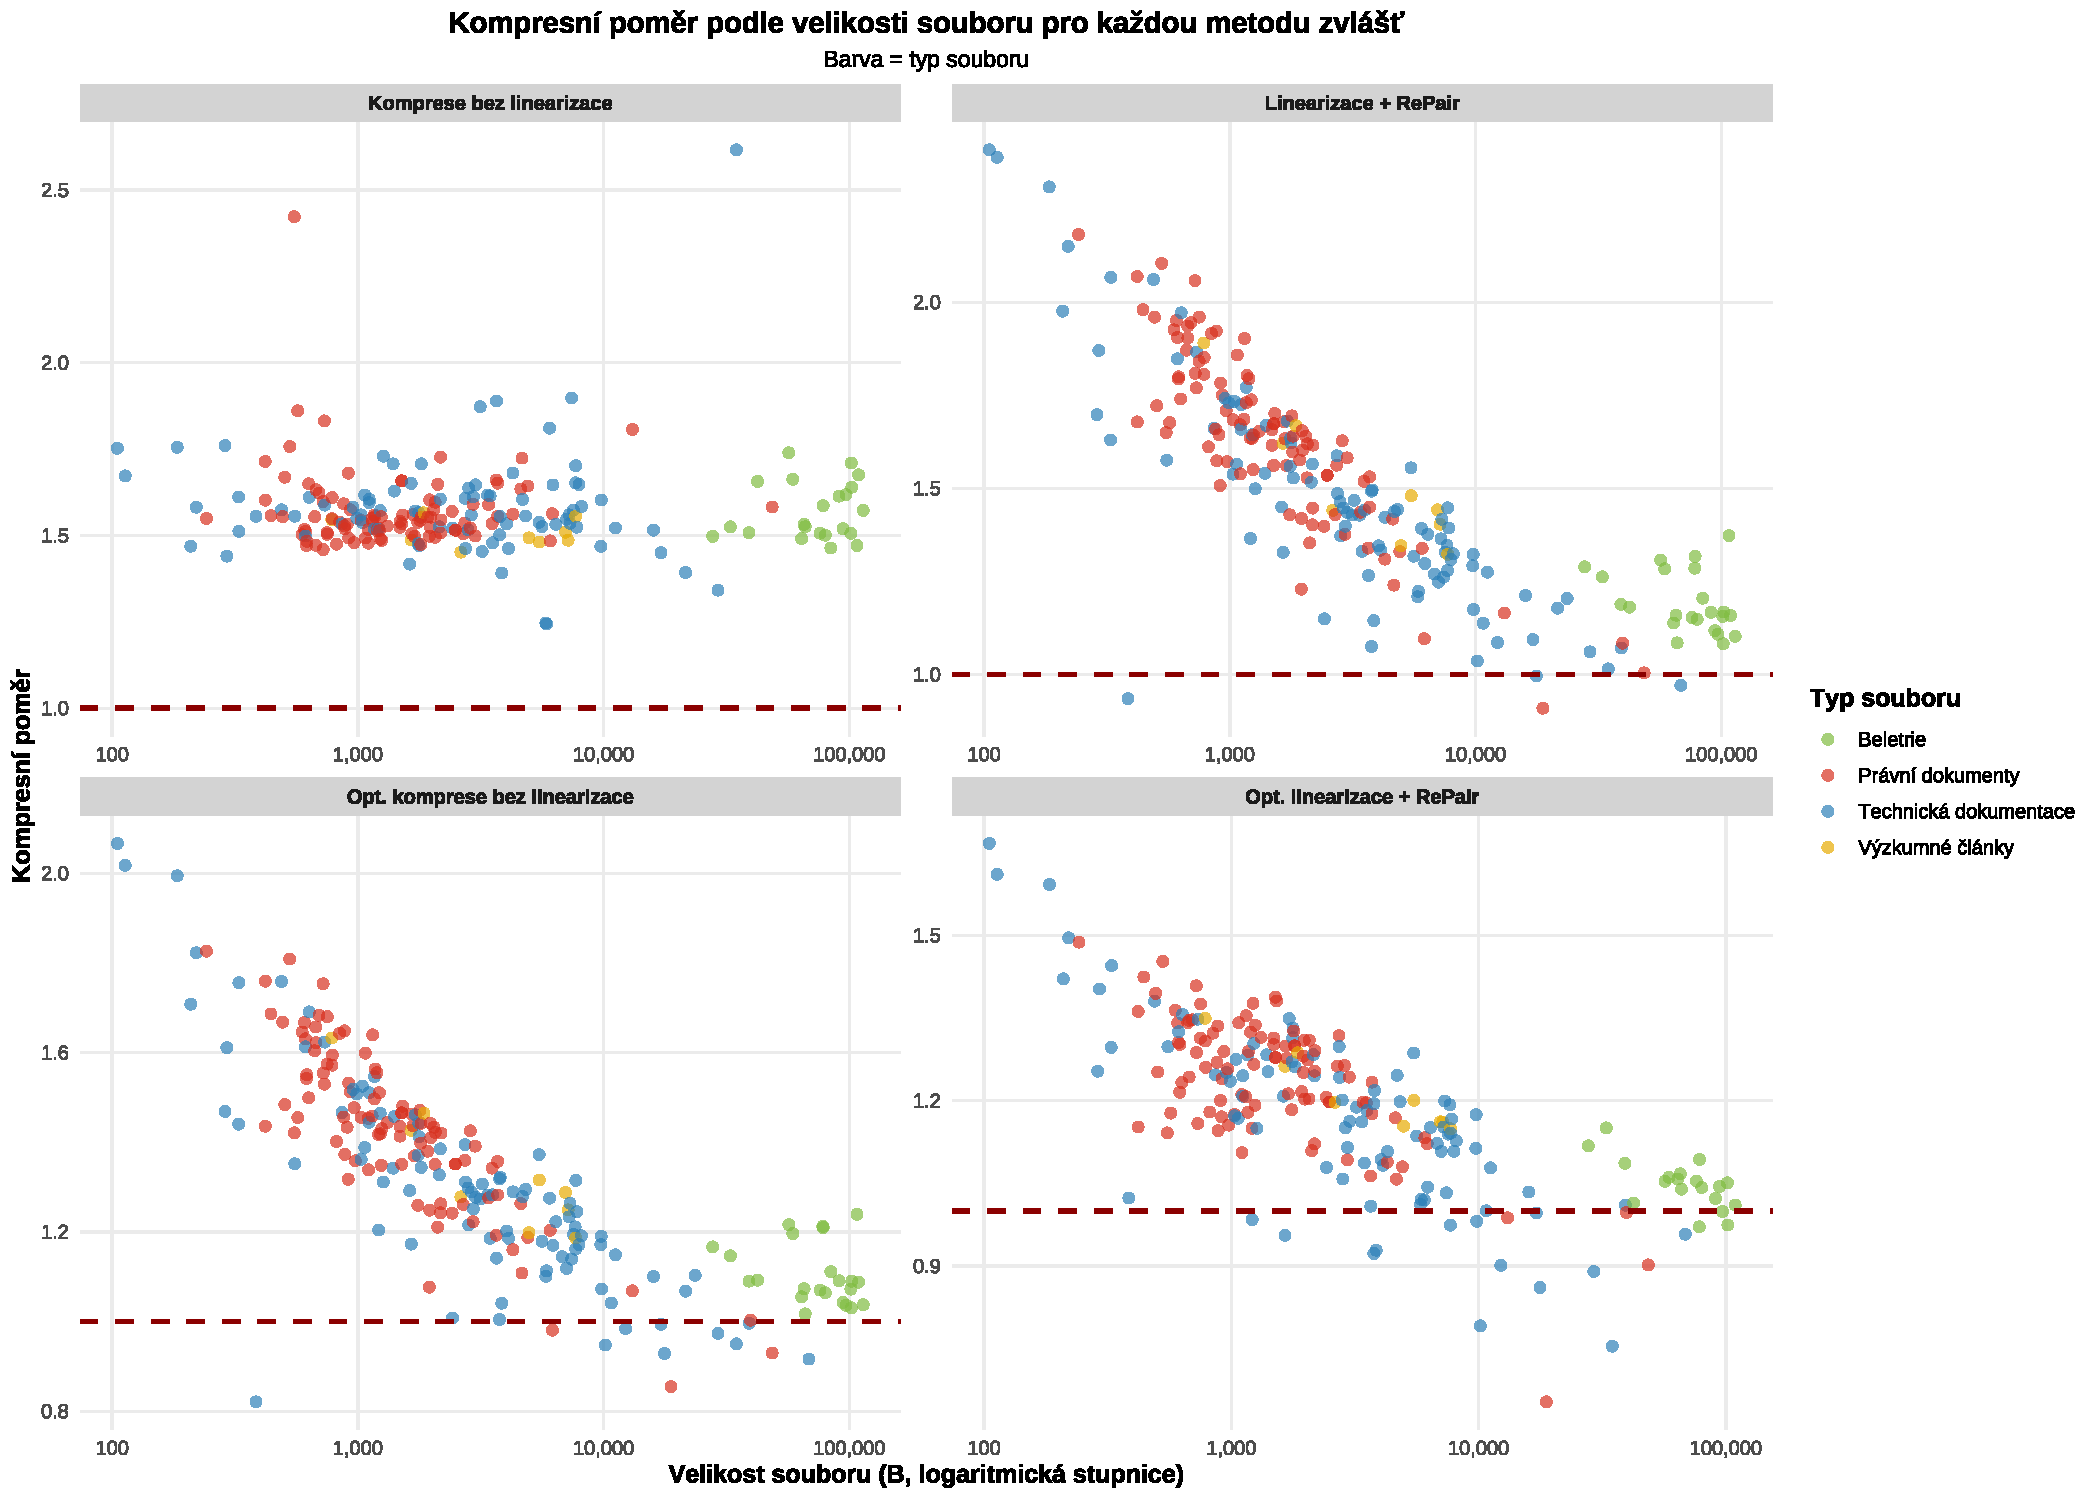
\includegraphics[width=\textwidth]{fig/compression_ratio_by_size_per_method.pdf}
    \label{fig:compression_ratio_by_size_per_method}
  \end{figure}
\end{frame}


\begin{frame}
  \begin{figure}
    \centering
    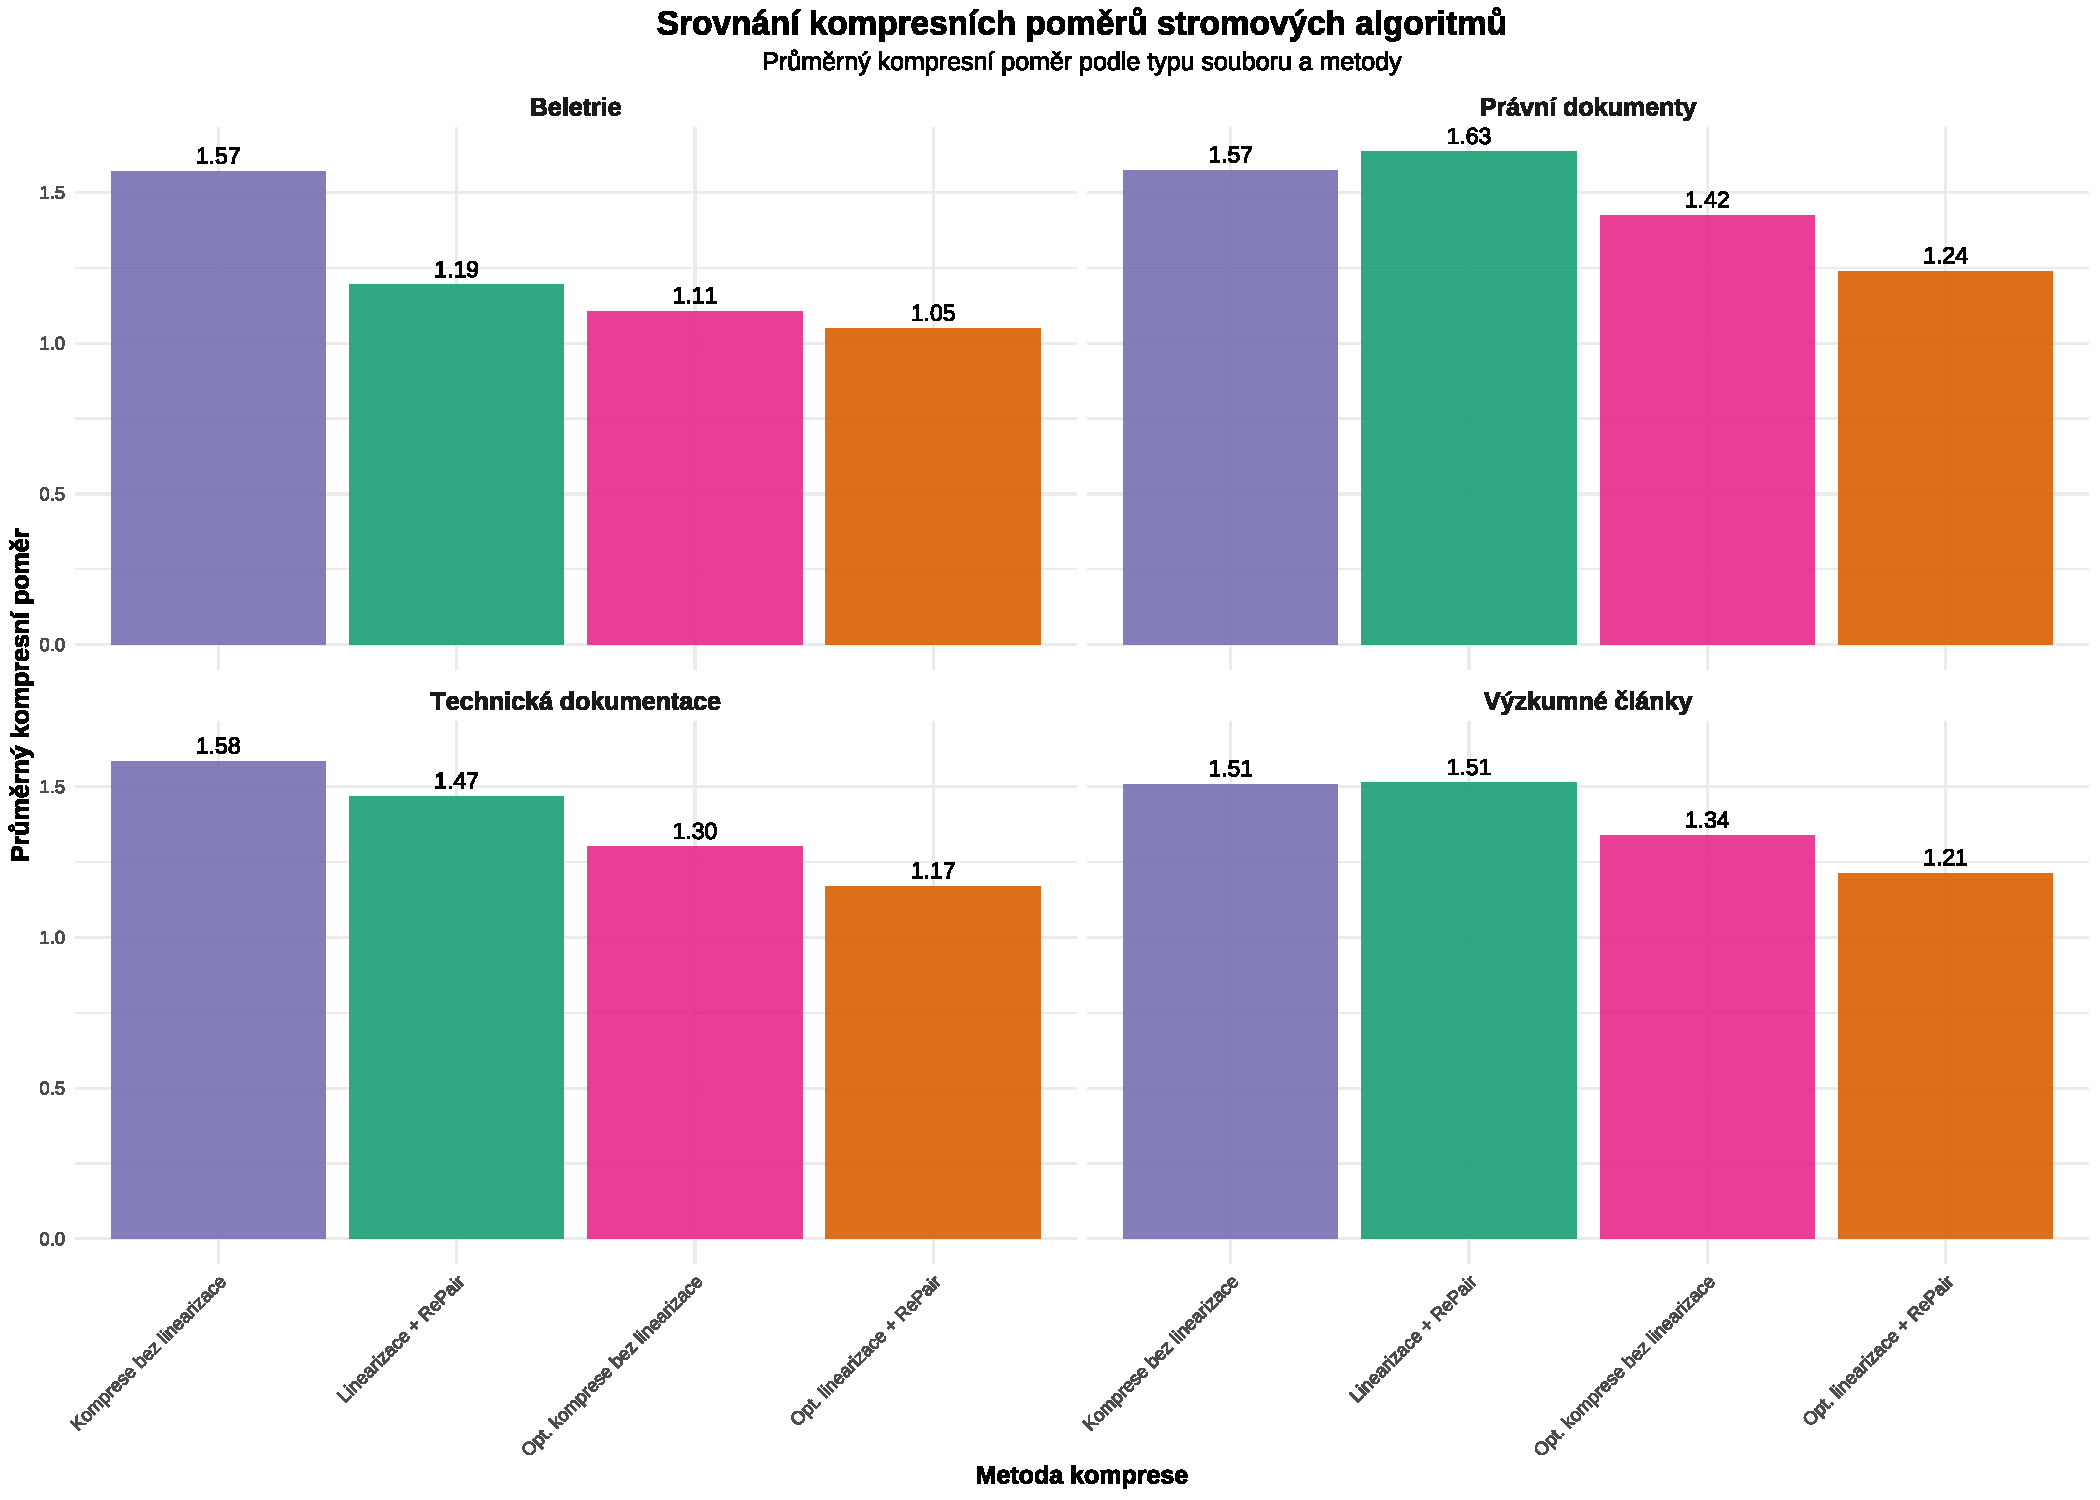
\includegraphics[width=\textwidth]{fig/presentation_overview.pdf}
    \label{fig:presentation_overview}
  \end{figure}
\end{frame}

\section{Literatura}
\begin{frame}[allowframebreaks]
    \frametitle{Literatura}
    \printbibliography[heading=none]
\end{frame}

\end{document}